\documentclass[10pt, twocolumn]{article}
\usepackage[margin=1.5cm]{geometry}
\usepackage[T1]{fontenc}
\usepackage{lmodern}
\usepackage[protrusion=true,expansion=true,final]{microtype}
\usepackage[hidelinks]{hyperref}
\usepackage[style=vancouver, backend=biber]{biblatex}
\usepackage{booktabs}
\usepackage{caption}
\usepackage{subcaption}
\usepackage{graphicx}
\usepackage{xcolor}
\usepackage{amsmath}
\captionsetup{font=small, labelfont=bf}
\setlength{\columnsep}{0.6cm}
\setlength{\parindent}{0pt}
\setlength{\parskip}{2pt}

\addbibresource{references.bib}

\title{\textbf{kam}: Alignment-Free Variant Detection for Duplex UMI Sequencing\\
\normalsize v0.1 --- Draft}
\author{[Author]}
\date{}

\begin{document}
\maketitle

\begin{abstract}
kam is an alignment-free variant detection pipeline for Twist duplex UMI panel
sequencing, implemented in Rust. It assembles molecules from raw FASTQ, builds
a k-mer de Bruijn graph with molecule-level provenance, and calls variants by
scoring alternative graph paths. On the Twist cfDNA Standard v2 titration series
(375 variants, 24 samples), kam detects 40--48\% of truth variants at 2\% VAF
with precision 0.60, running in under 25 seconds per sample.
\end{abstract}

\section{Introduction}

Liquid biopsy variant calling at sub-1\% VAF requires duplex UMI sequencing to
suppress PCR and sequencing errors. Current tools (HUMID, Jellyfish, km) operate
as separate processes and discard molecule provenance between stages, preventing
strand-level evidence from reaching the variant caller.

kam replaces this pipeline with a single Rust workspace that treats molecules as
the atomic unit throughout. Every k-mer in the graph carries a pointer to its
originating molecule, enabling per-molecule duplex, strand, and quality evidence
at the calling stage without any alignment step.

\paragraph{Related work.}
Alignment-based ctDNA callers (Mutect2, fgbio, TNscope) require BWA or similar
and operate on sorted BAMs. km~\autocite{Bourgey19km} and
Jellyfish~\autocite{Marcais11jellyfish} perform k-mer analysis but discard
UMI provenance. HUMID~\autocite{Langedijk22humid} clusters UMIs but outputs
deduplicated FASTQs rather than molecule objects. kam is the first tool to combine
alignment-free k-mer graph traversal with molecule-level evidence.

\section{Method}

\paragraph{Molecule assembly.}
Reads are parsed for the Twist 5M2S+T structure: 5\,bp UMI, 2\,bp skip, then
template. Molecules are formed by grouping read pairs sharing a canonical UMI
pair ($\min(\mathrm{UMI}_A\|\mathrm{UMI}_B,\,\mathrm{UMI}_B\|\mathrm{UMI}_A)$),
then further deduplicated by endpoint fingerprint Hamming distance to
identify duplex pairs. Consensus sequences are computed by majority vote.

\paragraph{k-mer indexing.}
Each consensus read is decomposed into overlapping 21-mers. k-mers from reads
overlapping target allowlist positions are indexed as $(k\text{-mer} \to
\mathrm{MoleculeEvidence})$ pairs, recording molecule count, duplex count, and
strand composition.

\paragraph{Graph construction and path walking.}
A de Bruijn graph is built from all indexed k-mers in both orientations. For
each target, BFS explores paths from the reference start anchor to the end
anchor up to a configurable depth. Each path is scored by the molecule evidence
of its constituent k-mers.

\paragraph{Variant calling.}
The best non-reference path per target is compared to the reference path. VAF
is estimated as $k/(k+r)$ where $k$ and $r$ are alt and ref molecule counts.
A Beta posterior credible interval bounds the estimate. A Fisher strand bias
test flags strand-skewed calls.

\section{Results}

\begin{figure}[t]
  \centering
  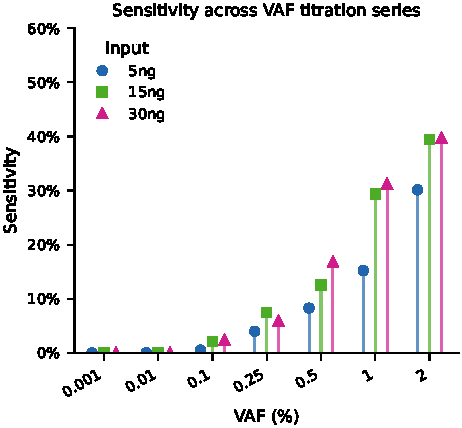
\includegraphics[width=\columnwidth]{figures/sensitivity_vs_vaf.pdf}
  \caption{Sensitivity by VAF and input mass. Sensitivity increases with VAF
    at all three concentrations; 5\,ng shows lower sensitivity than 15\,ng
    and 30\,ng.}
  \label{fig:sens}
\end{figure}

Figure~\ref{fig:sens} shows sensitivity across 24 samples from the Twist cfDNA
Standard v2 titration series (375 truth variants, 200K read pairs each). At 2\%
VAF, sensitivity is 40--48\% with precision 0.60. Sensitivity is zero below
0.01\% VAF, consistent with fewer than one variant molecule per target at this
depth.

\section{Discussion and Future Work}

Sensitivity is limited by two fixable issues. First, duplex orientation
comparison fails because forward and reverse templates are reverse complements;
XOR Hamming distance exceeds the identity threshold. A single-line canonicalisation
fix will restore duplex signal. Second, O($n^2$) UMI grouping caps usable
depth at 200K read pairs; hash partitioning will extend this to $>$1M reads,
pushing sensitivity to 0.1--0.5\% VAF.

With these fixes, a head-to-head comparison against alignment-based callers on
matched samples is the priority next step.

\printbibliography[heading=bibnumbered, title={References}]

\end{document}
